\section{Forward Flux sampling}

Computational methods are used to study a wide variety of phenomena, ranging from
large meteorological events to chemical reactions at the atomic scale. One class of
phenomena that is omnipresent in all these fields are the rare events. A rare event is an
event caused by stochastic fluctuations in the system, characterised by a large
difference in the time-scales corresponding to the duration of the events and their
temporal spacing. The infrequency of their occurrence in combination with their short
duration, makes them hard to study with both experimental and computational approaches.

Using this definition, the hybridisation and toehold displacement reactions studied in
this thesis can be classified as a rare event. Due to
the large temporal spacing of these rare events, simulating them with a brute-force
approach is inefficient. In this case, molecular dynamics simulations spend a lot of
computational resources on simulating the waiting time between events. To
effectively probe the kinetics of these rare events, advanced sampling methods are
needed.

A large ensemble of advanced sampling methods have been developed and can be largely
divided into two classes. The first class encompasses the free energy methods, based upon
applying a biasing potential onto chosen collective variables. These potentials bias the
Hamiltonian of the system in such a way, that rare parts of its configurational space are
explored. Notable examples of these methods are the adaptive biasing force algorithm[.],
basis function sampling[.] and umbrella sampling[.]. %(SSAGES)

The second class of methods, known as path sampling methods, do not influence the
systems Hamiltonian, but rather interface directly with the simulated trajectories. The
transition path ensemble is usually sampled by perturbing an initial transition path or
partitioning the phase space in subregions. Examples of these methods are transition
path sampling[.] and forward flux sampling[.][.]. The latter will be used in our
hybridisation simulations, motivated by its relative simplicity.

Forward Flux Sampling (FFS) starts with identifying two local minima, $A$ and $B$, in the
energy landscape of our system, for which we want to sample the transition path ensemble.
Next an order parameter, $\lambda(x)$, is defined with the aim of partitioning the
phase space, $\Omega$, using a set of nonintersecting hypersurfaces. By design, we
choose this order parameter to be a function, $\lambda(.):\ $\Omega$\ \rightarrow
\mathcal{R}$, monotonically increasing from the initial state $A$ to the final
state $B$.

Using this function the two local minima can
now be specified as $A := \{x: \lambda(x) < \lambda_A\} $ and $B := \{x: \lambda(x) \geq
\lambda_B\} $. The chosen levels of order, $\lambda_A$ and $\lambda_B$, construct the
interfaces separating the two local energy basins from the rest of the
phase space. Finally, this procedure can be done for a $N$-number of interfaces
partitioning the space between $A$ and  $B$, for which we require
\begin{equation}
\lambda_A = \lambda_0 < \lambda_1< \dots < \lambda_{N-1} < \lambda_N = \lambda_B.
\end{equation}
Note that this method does not require an in depth knowledge of the systems energy
landscape, however the choice of order parameter will heavily influence the
efficiency of the simulation. Analogous to the ambiguous choice of a collective variable
in free energy methods, constructing these hypersurfaces is often more an art then a
science.

The ultimate aim of these methods is to get a grasp of the kinetics of rare events. In
quantitative terms this means determining the rate constant of the transition
from $A$ to  $B$, denoted as $k_{AB}$. The expression used to calculate $k_{AB}$ is:
 \begin{equation}
    k_{AB} = \frac{\langle \Phi_{A,n} \rangle}{\langle h_{\mathcal{A}}\rangle} =
    \frac{\langle \Phi_{A,0} \rangle}{\langle h_{\mathcal{A}}\rangle}
    P(\lambda_n|\lambda_0),
 \end{equation}
 where $\langle \Phi_{A,n} \rangle$ is the steady-state flux of trajectories starting in
 $A$ and reaching the final interface $\lambda_n$ (i.e. reaching B) and
$\langle h_{\mathcal{A}}\rangle$ is the average fraction of time that  a trajectory
spends in the basin of local minima $A$. In the above equation this steady state flux is
factorised into the flux of trajectories starting in $A$ and crossing $\lambda_0$ and the
subsequent probability of reaching the final state from this
interface. Using the previously defined interfaces, we can now factorise the events'
probability into transition probabilities between the individual interfaces as
\begin{equation}
    P(\lambda_n|\lambda_0) = \prod_{i=0}^{n-1} P(\lambda_{i+1}|\lambda_i).
 \end{equation}
Estimating these transition probabilities can be done by shooting trajectories starting
from one interface to the next, while keeping track of the fraction of attempts
successfully crossing the next interface. Since not the entire energy landscape between
the minima has to be crossed, measuring these small transitions can be more easily done.

Note that this set-up allows for simulations of both equilibrium and out-of-equilibrium
systems, since it does not require detailed balance like other sampling techniques.
Non-equilibrium systems are ubiquitous in soft matter physics, illustrating another
strength of the method.
\begin{figure}[ht]
\begin{center}
  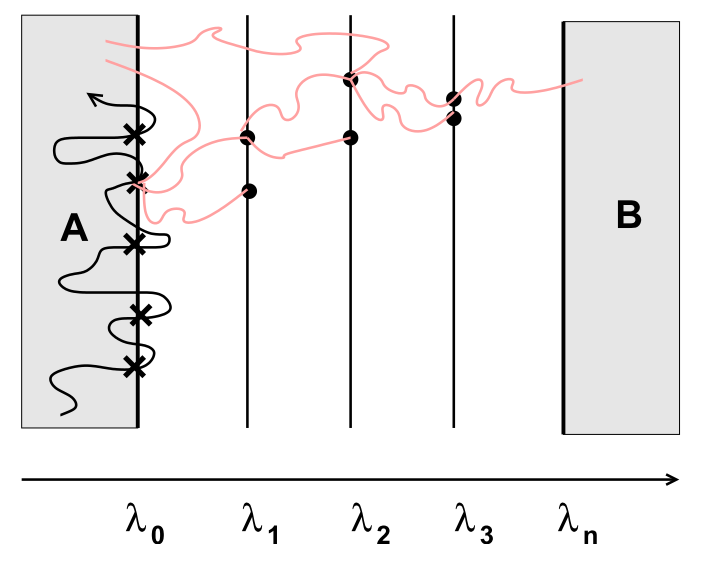
\includegraphics[width=0.5\textwidth]{Figures/FFS.png}
  \caption{write caption[.]}
\end{center}
\end{figure}
Different variants on the FFS method have been devised, differing in the approach by
which they calculate the probability $P(\lambda_n|\lambda_0)$. During this thesis I
chose to use the “Rosenbluth-like” (RB) method [zie citation allen review]. The choice
is motivated
by its resemblance with well known Monte Carlo Simulations and recursive nature, making
it easy to implement.  This method generates unbranched transition paths from state $A$
to state $B$, making them easy to analyse. The algorithm is described in six steps:
\begin{enumerate}[label=\textbf{(\roman*)}]
   \item Generate configurations on the $\lambda_0$ interface by running
      simulations in the $A$ basin. Keeping track of the fraction of successful runs,
      $\langle\Phi_{A,0} \rangle/\langle h_{\mathcal{A}}\rangle$ is evaluated.
   \item Fire $k_0$ trial runs from generated configurations on $\lambda_0$ until they
      cross $\lambda_1$ or cross back to $\lambda_0$. Store the final configurations of
      the successful simulations.
   \item Sample one of the saved configuration on the $\lambda_1$ interface and use it to
      shoot $k_1$ runs to the next interface $\lambda_2$.
   \item Iterate the previous steps until the trajectories reach $\lambda_n$ or no more
     configurations are available.
   \item If not successful, sample a stored configuration on $\lambda_0$ and repeat the
      steps $\textbf{(i)}$ to $\textbf{(iv)}$.
   \item Finally compute $P(\lambda_n|\lambda_0)$ using a weighted average of individual
     transition probabilities as described below.
\end{enumerate}
Calculating the transition probabilities is done by taking a weighted average of the
attempted trial runs. The path $b$ starting at the initial basin and reaching
interface $\lambda_i$ is assigned a weight $w_{i,b}$ as
\begin{equation}
   w_{i,b} = \prod_{j=0}^{i-1} S_{j,b}/k_j,
\end{equation}
where $S_{j,b}$ is the number of successful trajectories crossing interface $j$ during
the generation of path $b$. Using these weights, the transition probability is computed
using
\begin{equation}
   P(\lambda_{i+1} | \lambda_i) = \frac{\sum_{b} w_{i,b}\ S_{i,b}/k_i}{\sum_b w_{i,b}}.
\end{equation}

